\documentclass[convert={density=300,size=1080x800,outext=.png}]{standalone}
\usepackage{xcolor}
\usepackage{graphics, graphicx}
\usepackage{tikz, tkz-graph}
\usepackage{pgf, pgfplots}
\usepackage{graphviz, tkz-berge}
\usepackage{graphics, graphicx}
\usepackage{pstricks, pst-node, pst-tree}

\usetikzlibrary{arrows, petri, topaths}
\usetikzlibrary{shapes}
\usetikzlibrary{arrows.meta}
\usetikzlibrary{positioning,automata}



\begin{document}
		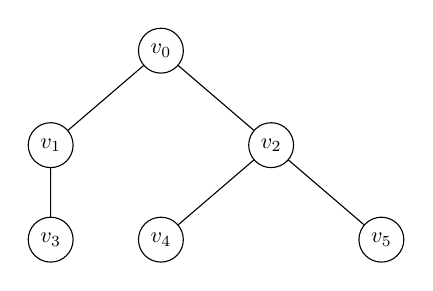
\begin{tikzpicture}[round/.style={circle, draw=black, thin, minimum 			size=.5mm}, transform shape, scale=0.80]
			\tikzstyle{level 1}=[level distance=15mm,sibling distance=35mm]
			\node(0)[round]{$v_{0}$}
				child{node[round]{$v_{1}$}
					child{node[round]{$v_{3}$}}}
				child{node[round]{$v_{2}$}
					child{node[round]{$v_{4}$}}
					child{node[round]{$v_{5}$}}
			};
		\end{tikzpicture}
\end{document}